\documentclass[Main]{subfiles}
\begin{document}

\chapter{Hardware}

\section{System oversigt}

Til styring af drone, skal der laves en sender og modtager.

\begin{figure}[H]
\centering
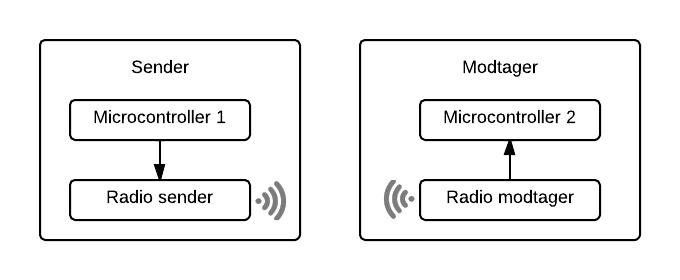
\includegraphics[scale=0.6]{Blokdiagram}
\caption{Skitse af hardware}
\end{figure}

\code{Senderen} er den brugeren laver sit indput på. 
\\ \code{Modtageren} er den enhed der er sat på dronen, som skal modtage signalet fra senderen.\\
Det vil sige der skulle laves to enheder. Begge skulle gøre brug af chippen cc1101 fra texas instruments. Og microcontrolleren atmega8 fra Atmel Corporation.
\code{Senderen} skal også have knapper så brugeren kan lave sit indput.

\section{Grænseflader}

De interne og eksterne grænseflader. 

\subsection{Sender}
\begin{figure}[H]
\centering
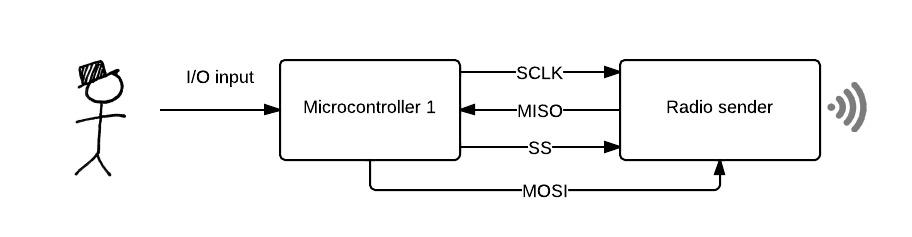
\includegraphics[scale=0.5]{SenderInterface}
\caption{Grænseflader for sender}
\label{fig: SenderInterface}
\end{figure}

På Figur \ref{fig: SenderInterface} ses et blokdiagram af senderen med alle grænseflader.

De eksterne grænseflader, er der hvor brugeren skal lave sit indput. Det vil sige der er her han laver et programvalg som bliver sendt videre til dronen.

De interne grænseflader
Kommunikationen mellem microcontroller 1 og radiosenderen, forgår via SPI protokollen. 

Radio interfacet er beskrevet i sektionen Radio.



\subsection{Modtager}

\begin{figure}[H]
\centering
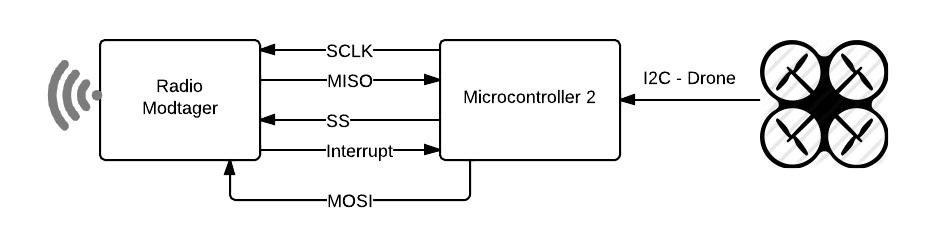
\includegraphics[scale=0.5]{ModtagerInterface}
\caption{Grænseflader for modtager}
\label{fig: ModtagerInterface}
\end{figure}
På Figur \ref{fig: ModtagerInterface} ses et blokdiagram af modtageren med alle grænseflader.
Radioen modtager en pakke fra senderen. Når hele pakken er modtaget laves et interrupt på microcontroller 2.

Microcontroller 2, henter hele pakken fra radioen og sætter den i modtage mode igen. 

Microcontroller 2, tager så de modtaget data fra radioen og putter dem i en output buffer til \itoc.

Radio interfacet er beskrevet i næste sekstion.


\subsection{Radio}
Opsætningen på radioen vi køre med er som følger:

\begin{itemize}
\item 433MHz
\item 2.5 kbps
\item CRC af dataoverførslen
\item Benytter kanal 0
\end{itemize}

Pakken der bliver sendt frem og tilbage ser ud som følger:
\begin{figure}[H]
\centering
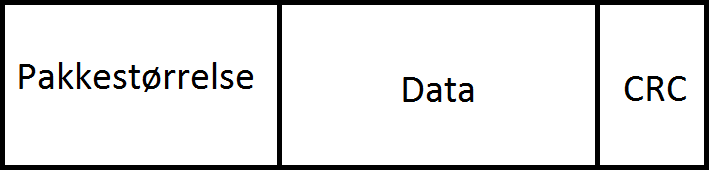
\includegraphics[scale=0.8]{Pakke}
\caption{Pakke opbygningen}
\label{fig: Pakke}
\end{figure}
\section{Design}

Hastigheden SPI interfacet køre med er:
$ \dfrac{8.000.000 Hz}{16} = 500.000Hz $

\itoc hastighed

Tach Switch som bruger indput

Radiosender sender med en frekvens 

\subsection{Strøm indput}

Hele enheden køre på 3.3 V.
Der er ikke lavet noget beskyttelse på inputstrømmen så det skal være 3.3V dc.

\section{PCB layout}

\begin{figure}[H]
\centering
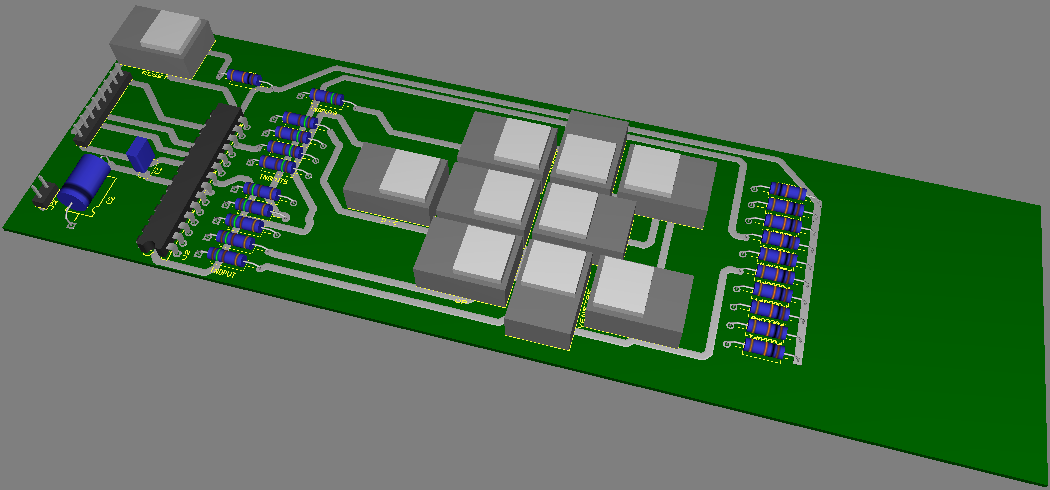
\includegraphics[scale=0.5]{Print3D}
\caption{Det færdige print}
\label{fig: Print3D}
\end{figure}

Layouted er forsøgt holdt simpelt. knapperne til brugeren er placeret så de minder om pilene på et tastatur, dog med op/ned funktioner og autoland.
Printet er aflangt så det er til at holde som en fjernbetjening og derved kan styres med en hånd.
Radioen er placeret forrest på fjernbetjeningen, for at brugeren dæmper/skærmer mindst muligt for signalet.  

Opdeling i blokke.
Interface mellem blokkene, f.eks.:
Realisering af den enkelte blok
· Enhedstest af den enkelte blok

Analoge/digitale niveauer
o Impedanser,
o Protokol (f.eks. mellem PC og mikroprocessor)



\end{document}